\section{Segunda Captura: Red local chica}

\begin{figure*}[h]
  \hspace*{-0.5cm}
  \begin{subfigure}{1.1\textwidth}
    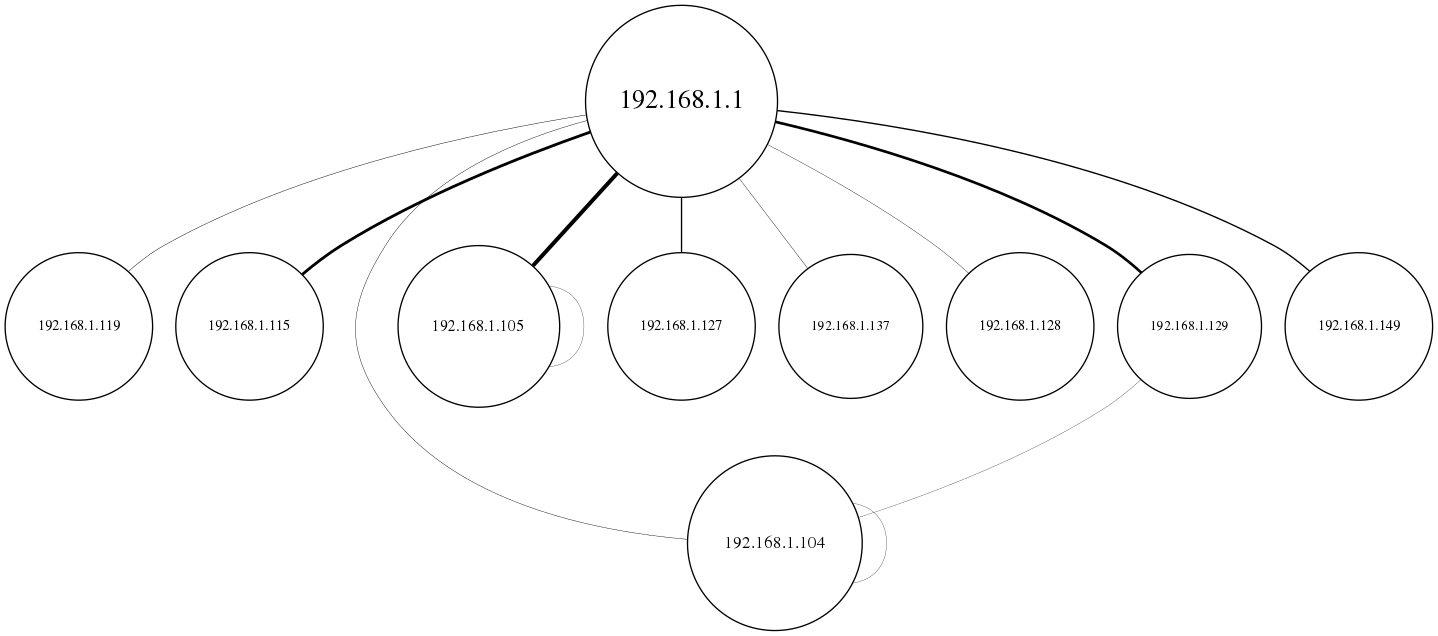
\includegraphics[width=\textwidth]{imagenes/hogarenia/grafo.png}
  \end{subfigure}
	\label{fig:expw_hogar_grafo}
	\caption{Grafo con los nodos de la red de la segunda captura. El diámetro del nodo implica mayor participación en el envío de paquetes.}
\end{figure*}

\begin{figure}[h]
  \begin{subfigure}{.5\textwidth}
    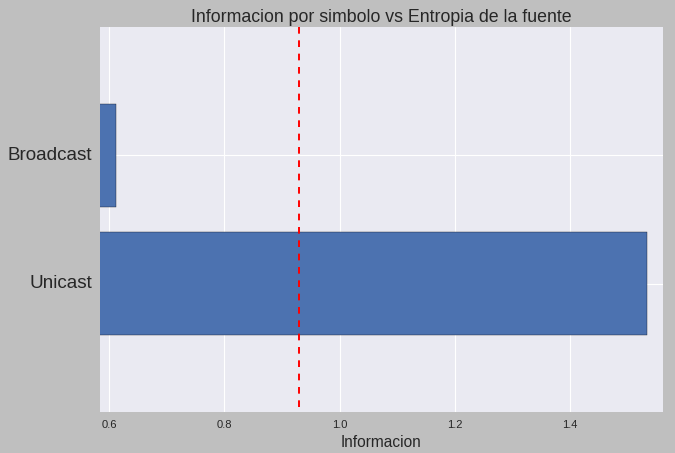
\includegraphics[width=\textwidth]{imagenes/hogarenia/brvsun_informaciones_vs_entropia.png}
  \end{subfigure}
  \label{fig:exp2_hogar_brvsun_infovsentro}
  \caption{Información de cada símbolo (Broadcas / Unicast) comparada con el valor de la entropía de la fuente de información (red local).}
\end{figure}

\begin{figure}[h]
  \begin{subfigure}{.5\textwidth}
    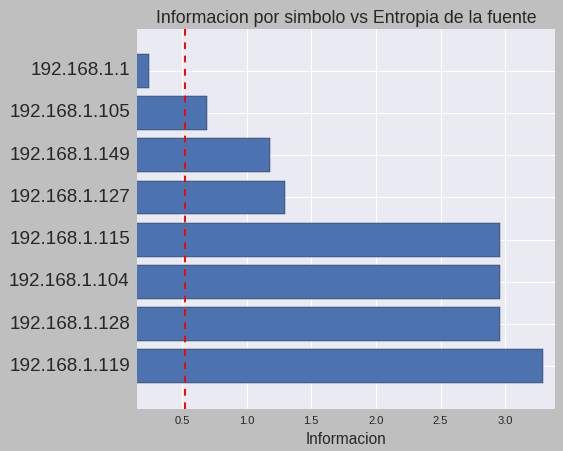
\includegraphics[width=\textwidth]{imagenes/hogarenia/hosts_informaciones_vs_entropia.png}
  \end{subfigure}
  \label{fig:exp2_hogar_hosts_infovsentro}
  \caption{Información de cada símbolo (host) comparada con el valor de la entropía de la fuente de información (red local).}
\end{figure}

\\
\newpage
